\documentclass[../../../../main.tex]{subfiles}
\usepackage{tikz}
\usepackage{amsmath,amssymb}
\begin{document}
\section*{東大理科数学 2009年}
ビジョーダナ
\begin{center}
\begin{tabular}{|c|l|c|c|c|}
\hline
& & け & 思 & 続 \\
\hline
\fbox{1} & セイスウ & A & c & c \\
\hline
\fbox{2} & 行列 & & & \\
\hline
\fbox{3} & 場数 & B & A & B \\
\hline
\fbox{4} & 空間 & B & B & B \\
\hline
\fbox{5} & 不等式 & B & B & B \\
\hline
\fbox{6} & 多変数 & C & B & c \\
\hline
\end{tabular}
\end{center}

\subsection*{第1問}
[解] $m \ge 2 \cdots (1)$

$d_m$ は $mC_1$ を割り切ることが必要で、すなわち $d_m$ は $m$ の約数である $\cdots (2)$

(1) $m \in \text{prime}$ の時、(2) から $d_m = 1 \text{ or } m$ である。以下、$k=2,\dots,m-1$ に対し、
${}_{m}C_{k}$ が $m$ で割り切れることを示す。
\[
k \cdot {}_{m}C_{k} = m \cdot {}_{m-1}C_{k-1} \quad \therefore \quad {}_{m}C_{k} = \frac{{}_{m-1}C_{k-1}}{k} \cdot m
\]
ここで、$m$ と $k$ は互いに素で、かつ ${}_{m}C_{k} \in \mathbb{N}$ だから、$\frac{{}_{m-1}C_{k-1}}{k} \in \mathbb{N}$ となり、
たしかに ${}_{m}C_{k}$ は $m$ の倍数\fbox{終}

以上から、$d_m = m$ が従う\fbox{終}

(2) $k=1$ の時は成立するから、以下 $k=i \in \mathbb{N}$ での成立を仮定し、$k=i+1$ での成立を示す。$a_m(k) = k^m - k$ とおく。
\begin{align*}
a_m(i+1) &= (i+1)^m - (i+1) = \sum_{t=0}^{m} {}_{m}C_{t} \cdot i^t - i - 1 \\
&= \sum_{t=1}^{m-1} {}_{m}C_{t} \cdot i^t + (i^m - i)
\end{align*}
ここで、${}_{m}C_{t}$、$i^m - i$ は共に $d_m$ で割り切れるので、$a_m(i+1)$ も $d_m$ で割り切れる。
よって $k=i+1$ でも成立し、以上から題意は示された\fbox{終}

(3) $(1-1)^m = \sum_{k=0}^{m} {}_{m}C_{k} (-1)^k = 2 + \sum_{k=1}^{m-1} {}_{m}C_{k} (-1)^k = 0 \quad (\because m \in \text{even}) \cdots (3)$

${}_{m}C_{k} \ (k=1,2,\dots,m-1)$ は $d_m$ で割り切れるので、$S \in \mathbb{Z}$ として、(3) から
\[
d_m \cdot S = 2
\]
とかける。$d_m \in \mathbb{N}$ から、$d_m = 1 \text{ or } 2$ が従う。\fbox{終}

\subsection*{第2問}
(解答なし)

\subsection*{第3問}
[解] (1) 1に4色すべてが入っている確率を $\alpha$ とすると、対称性から、求める確率 $P_1$ は
\[
P_1 = \alpha^2 \cdots (1)
\]
である。$\alpha$ について、5回の操作で、4つの色のうち、3つの色が1回ずつ、の残りの1色が2回出るので、
\[
\alpha = 4 \cdot {}_5C_2 \cdot {}_3C_1 \cdot {}_2C_1 \cdot \left(\frac{1}{4}\right)^5 = \frac{15}{4^3}
\]
だから、(1)より
\[
P_1 = \frac{3^2 \cdot 5^2}{4^6} \quad \text{\#\!}
\]

(2) 5回の操作で、4色全てが少なくとも1回出れば良く、$P_2 = \alpha = \frac{3 \cdot 5}{4^3} \quad \text{\#\!}
\]

(3) 10回の操作で、4色全てが少なくとも2回出れば良い。この時、残りの2つの玉について、
\begin{itemize}
\item[$1^\circ$] 2つとも同じ色
\item[$2^\circ$] 2つとも違う色
\end{itemize}
がありうる。$1^\circ$ の時の確率は
\[
4 \times {}_{10}C_{4} \cdot {}_{6}C_{2} \cdot {}_{4}C_{2} \cdot \left(\frac{1}{4}\right)^{10} = 3^3 \cdot 5^2 \cdot 7 \left(\frac{1}{4}\right)^8
\]
$2^\circ$ の時の確率は
\[
{}_{4}C_{2} \cdot {}_{10}C_{3} \cdot {}_{7}C_{3} \cdot {}_{4}C_{2} \cdot \left(\frac{1}{4}\right)^{10} = 3^3 \cdot 5^2 \cdot 7 \cdot 2 \left(\frac{1}{4}\right)^8
\]
だから、
\[
P_3 = 3^3 \cdot 5^2 \cdot 7 \cdot \left(\frac{1}{4}\right)^8 (1+2) = 3^4 \cdot 5^2 \cdot 7 \left(\frac{1}{4}\right)^8
\]
(1)とあわせて、
\[
\frac{P_3}{P_1} = \frac{4^6 \cdot 3^4 \cdot 5^2 \cdot 7}{3^2 \cdot 5^2 \cdot 4^8} = \frac{3^2 \cdot 7}{4^2} = \frac{63}{16} \quad \text{\#\!}
\]

\subsection*{第4問}
[解] 対称性から、$y \ge 0$ で考える。以下
$C: x = 0, \ z = \sin \theta \text{ を表す。} y = S \ (0 \le \theta \le \pi/2)$
で、$D_1$ を切断すると $z = a, \ |x| \le c$ となる
から、この部分を $y$ 軸まわりに回した時の
根元形は右下図のようになる。このうち、
$x \ge 0$ をみたす部分の面積 $S(\theta)$ は
\[
S(\theta) = \frac{1}{2}\pi \left[ (a^2+c^2) - a^2 \right] = \frac{1}{2}\pi c^2
\]
だから、対称性から
\begin{align*}
\frac{1}{2} W(a) &= \int_{0}^{s} S(\theta) ds \\
&= \int_{0}^{\pi/2} \frac{1}{2}\pi c^2 \frac{ds}{d\theta} d\theta \\
&= \frac{1}{2}\pi \int_{0}^{\pi/2} c^3 d\theta \\
&= \frac{1}{2}\pi \int_{0}^{\pi/2} \left( \frac{3}{4}c + \frac{1}{4}c \cos 3\theta \right) d\theta \\
&= \frac{1}{2}\pi \left[ \frac{3}{4}s + \frac{1}{12}\sin 3\theta \right]_{0}^{\pi/2} = \frac{1}{2}\left(\frac{3}{4} - \frac{1}{12}\right)\pi = \frac{1}{3}\pi
\end{align*}
となって、
\[
W(a) = \frac{2}{3}\pi \quad \text{\#\!}
\]

\begin{center}
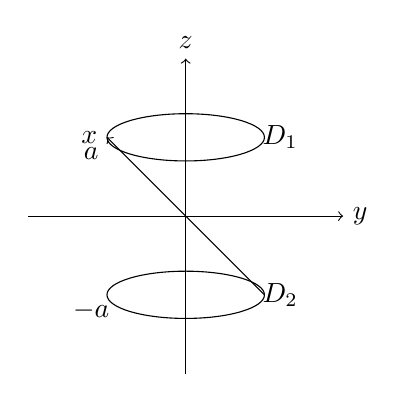
\begin{tikzpicture}
\draw[->] (-2,0) -- (2,0) node[right] {$y$};
\draw[->] (0,-2) -- (0,2) node[above] {$z$};
\draw[->] (1,-1) -- (-1,1) node[left] {$x$};
\draw (0,1) ellipse (1 and 0.3);
\draw (0,-1) ellipse (1 and 0.3);
\node at (1.2,1) {$D_1$};
\node at (1.2,-1) {$D_2$};
\node at (-1.2,0.8) {$a$};
\node at (-1.2,-1.2) {$-a$};
\end{tikzpicture}
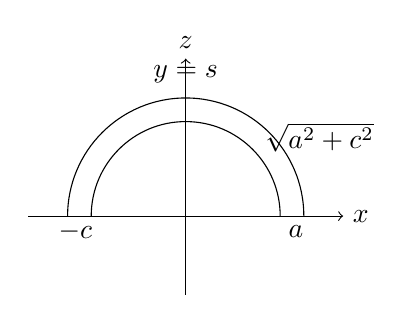
\begin{tikzpicture}
\draw[->] (-2,0) -- (2,0) node[right] {$x$};
\draw[->] (0,-1) -- (0,2) node[above] {$z$};
\draw (1.5,0) arc (0:180:1.5);
\draw (1.2,0) arc (0:180:1.2);
\node at (1.7,1) {$\sqrt{a^2+c^2}$};
\node at (1.4,-0.2) {$a$};
\node at (-1.4,-0.2) {$-c$};
\node at (0,1.8) {$y=s$};
\end{tikzpicture}
\end{center}

(2) $E$ のうち $x \le 0$ のものの $y=s$ における切断面の面積 $T(\theta)$ は、右上図から、
\begin{align*}
T(\theta) &= 2 \int_{-c}^{0} \left[ \sqrt{a^2+c^2-x^2} - a \right] dx \\
&= 2 \int_{0}^{c} \sqrt{a^2+c^2-x^2} dx - 2ac \quad \cdots (1)
\end{align*}
であり、
\[
V(a) = W(a) + 2 \int_{0}^{1} T(\theta) ds \quad \cdots (2)
\]
となる。ここで、$[0,c]$ において、$0 \le x^2 \le c^2$ だから、
\[
\sqrt{a^2} \le \sqrt{a^2+c^2-x^2} \le \sqrt{a^2+c^2}
\]
同区間で積分して、$a>0$ から
\[
\int_{0}^{c} a dx \le \int_{0}^{c} \sqrt{a^2+c^2-x^2} dx \le \int_{0}^{c} \sqrt{a^2+c^2} dx
\]
\[
ac \le \int_{0}^{c} \sqrt{a^2+c^2-x^2} dx \le c\sqrt{a^2+c^2} \quad \cdots (3)
\]
だから、(1)から、
\[
0 \le T(\theta) \le 2c \left[ \sqrt{a^2+c^2} - a \right]
\]
である。$[0,1]$ で積分して、
\[
0 \le \int_{0}^{s} T(\theta) d\theta \le 2 \int_{0}^{\pi/2} \left( c\sqrt{a^2+c^2} - ac \right) c d\theta \quad \cdots (5)
\]
ここで、(5)の右辺について $0 \le c^2 \le 1$ から、$c^2(\sqrt{a^2+c^2} - a) \le c^2(\sqrt{a^2+1} - a)$ に注意して、
\[
\int_{0}^{\pi/2} c^2(\sqrt{a^2+c^2} - a) d\theta \le (\sqrt{a^2+1} - a) \int_{0}^{\pi/2} c^2 d\theta = \cdots (6)
\]
(6)を(5)に代入して、$A = \int_{0}^{\pi/2} c^2 d\theta$ として、
\[
0 \le \int_{0}^{1} T(\theta) d\theta \le 2 \frac{1}{\sqrt{a^2+1} + a} A \quad \cdots (7)
\]
$A$ は $a$ に関係ない定数由、(7)の右辺は $a \to \infty$ で $0$ に収束する。これと(2)から、
はさみうちにより
\[
\int_{0}^{1} T(\theta) d\theta \to 0 \quad (a \to \infty)
\]
だから、(1)、(2)から $a \to \infty$ の時、
\[
V(a) \longrightarrow W(a) = \frac{2}{3}\pi \quad \text{\#\!}
\]

\subsection*{第5問}
[解] (1) $-1 < x < 1, \ x \ne 0 \cdots (1)$ から、与式の両辺正だから、
\[
(与式) \iff 1 - x < (1+x)^{\frac{1}{x}}(1-x)^{\frac{1}{x}} \quad \cdots (2)
\]
与式の両辺対数をとって、
\[
(1 - \frac{1}{x}) \log(1-x) < \frac{1}{x} \log(1+x) \quad \cdots (3)
\]
である。$f(x) = \log(1+x) - (x-1)\log(1-x)$ とおく。

$1^\circ \ 0 < x < 1$

(3)の両辺に $x$ をかけて
\[
(x-1) \log(1-x) < \log(1+x) \quad \cdots (4)
\]
である。よって $f(x) > 0$ を示せば良い。
\[
\begin{cases}
f'(x) = \frac{1}{x+1} - \log(1-x) - 1 \\
f''(x) = \frac{1}{1-x} - \frac{1}{(x+1)^2} = \frac{x(x+3)}{(x+1)^2(1-x)} \quad \cdots (5)
\end{cases}
\]
だから、$f''(x) > 0$ となって $f'(x)$ は単調増加。これと $f'(0) = 0$ から、$f'(x) > 0$ つまり
$f(x)$ も単調増加。よって、
\[
f(x) > \lim_{x \to +0} f(x) = 0
\]
だから(4)は示された。

$2^\circ \ -1 < x < 0$

両辺に $x$ をかけて、
\[
(x-1) \log(1-x) > \log(1+x) \quad \cdots (6)
\]
だから、$f(x) < 0$ を示せば良い。(5)から
\[
f''(x) < 0
\]
となり、$f'(x)$ は単調減少。これと $f'(0) = 0$ から、$f'(x) > 0$ つまり $f(x)$ は単調増加。
したがって
\[
f(x) < \lim_{x \to -0} f(x) = 0
\]
だから(6)は示された。

$1^\circ, 2^\circ$ から、与式は示された。\fbox{終}

(2) まず、(1)に $x = \frac{1}{100}$ ((1)をみたす) を代入して、
\[
0.99 < 0.9999^{100} \quad \cdots (7)
\]
又、与式の両辺に $(1+x)^{1-\frac{1}{x}}$ をかけて、
\[
(1-x^2)^{1-\frac{1}{x}} < 1+x
\]
$x = -\frac{1}{100}$ ((1)をみたす) として、
\[
0.9999^{101} < 0.99 \quad \cdots (8)
\]
(7)(8)から示された \fbox{終}

\subsection*{第6問}
[解]
(1) $\overrightarrow{OP_k(t)} = \overrightarrow{OA_k} + t \overrightarrow{e_k}$ だから、$(k=1,2,3)$
\begin{align*}
|\overrightarrow{P_1(t) P_2(t)}|^2 &= |\overrightarrow{OP_1(t)} - \overrightarrow{OP_2(t)}|^2 \\
&= \left| \overrightarrow{A_2 A_1} + t (\overrightarrow{e_1} - \overrightarrow{e_2}) \right|^2 \\
&= |-\overrightarrow{a_1} + t \overrightarrow{\alpha}|^2 \quad (\overrightarrow{\alpha} = \overrightarrow{e_1} - \overrightarrow{e_2}) \\
&= |\overrightarrow{a_1}|^2 + t^2 |\overrightarrow{\alpha}|^2 - 2t \overrightarrow{a_1} \cdot \overrightarrow{\alpha} \\
&= 10^2 + t^2 |\overrightarrow{\alpha}|^2 - 2t \cdot 1000 \cdot |\overrightarrow{\alpha}| \cdot \cos \theta \quad (0 \le \theta \le \pi) \quad \cdots (1)
\end{align*}
題意から、これが $1$ 以下になるような $t \ge 0$ があったので、
\[
|\overrightarrow{\alpha}|^2 t^2 - 2000 \cdot |\overrightarrow{\alpha}| \cos \theta \cdot t + 10^6 - 1 \le 0
\]
をみたす $t$ があった ($t>0$)。左辺 $f(t)$ として、$f(t)=0$ の判別式 $D$ とする。$\overrightarrow{\alpha} \ne 0$ から、
\[
\begin{cases}
D/4 \ge 0 \\
0 \le 1000 |\overrightarrow{\alpha}| \cos \theta
\end{cases} \iff
\begin{cases}
10^6 \cdot |\overrightarrow{\alpha}|^2 \cos^2 \theta - |\overrightarrow{\alpha}|^2 (10^6-1) \ge 0 \\
0 \le \cos \theta
\end{cases}
\]
\[
\iff
\begin{cases}
|\sin \theta| \le \frac{1}{10^3} \\
0 \le \cos \theta
\end{cases} \quad \cdots (2)
\]
から、たしかに $|\sin \theta| \le \frac{1}{10^3}$ である \fbox{終}

(2) (2)から、$0 \le \theta \le \alpha \cdots (3)$ である。この時、$\overrightarrow{a_1}$ と $\overrightarrow{\alpha}$ のなす角が $\theta$ だから、
\[
\cos \theta = \frac{\overrightarrow{a_1} \cdot \overrightarrow{e_1} - \overrightarrow{a_1} \cdot \overrightarrow{e_2}}{|\overrightarrow{a_1}| |\overrightarrow{\alpha}|} = \frac{10^3 \cos \theta_1 + 10^3 \cos(\theta_2 + \frac{2}{3}\pi)}{10^3 |\overrightarrow{\alpha}|} \quad \cdots (3)'
\]
さらに、$\overrightarrow{e_1}$ と $\overrightarrow{e_2}$ のなす角は $\frac{2}{3}\pi + \theta_2 - \theta_1$ だから
\begin{align*}
|\overrightarrow{\alpha}|^2 &= |\overrightarrow{e_1}|^2 + |\overrightarrow{e_2}|^2 - 2 \overrightarrow{e_1} \cdot \overrightarrow{e_2} = 2(1 - \cos(\frac{2}{3}\pi + \theta_2 - \theta_1)) \\
&= 4 \sin^2 (\frac{1}{3}\pi + \frac{\theta_2 - \theta_1}{2})
\end{align*}
ここで、$0 \le \theta_k \le \frac{\pi}{3}$ から、$\frac{\pi}{6} \le \frac{1}{3}\pi + \frac{\theta_2 - \theta_1}{2} \le \frac{\pi}{2}$ だから、$\cdots (4)$
\[
|\overrightarrow{\alpha}| = 2 \sin(\frac{1}{3}\pi + \frac{\theta_2 - \theta_1}{2})
\]
となり、(3)'に代入して、
\begin{align*}
2 \cos \theta &= \frac{\cos \theta_1 - \cos(\frac{2}{3}\pi + \theta_2)}{2 \sin(\frac{1}{3}\pi + \frac{\theta_2 - \theta_1}{2})} = \frac{-2 \sin(\frac{1}{3}\pi + \frac{\theta_1 + \theta_2}{2}) \sin(\frac{1}{3}\pi + \frac{\theta_2 - \theta_1}{2})}{\sin(\frac{1}{3}\pi + \frac{\theta_2 - \theta_1}{2})} \\
\therefore \sin(\frac{\pi}{2} - \theta) &= \sin(\frac{1}{3}\pi + \frac{\theta_1 + \theta_2}{2})
\end{align*}
(3)及び $\frac{1}{6}\pi \le \frac{1}{3}\pi + \frac{\theta_1 + \theta_2}{2} \le \frac{2}{3}\pi$ から、
\[
\frac{\pi}{2} - \alpha \le \frac{1}{3}\pi + \frac{\theta_1 + \theta_2}{2} \le \frac{\pi}{2} + \alpha
\]
\[
\therefore \frac{1}{3}\pi - 2\alpha \le \theta_1 + \theta_2 \le \frac{1}{3}\pi + 2\alpha \quad \text{\#\!}
\]
である。

(3) 対称性から、(2)と同様の式
\begin{cases}
\frac{1}{3}\pi - 2\alpha \le \theta_2 + \theta_3 \le \frac{1}{3}\pi + 2\alpha \\
\frac{1}{3}\pi - 2\alpha \le \theta_3 + \theta_1 \le \frac{1}{3}\pi + 2\alpha
\end{cases} \quad \cdots (6)
が成り立つ。
\[
\overrightarrow{OP_k(t)} = \overrightarrow{OA_k} + T \overrightarrow{e_k}
\]
だから
\begin{align*}
|\overrightarrow{OP_k(T)}|^2 &= |\overrightarrow{OA_k}|^2 + T^2 |\overrightarrow{e_k}|^2 + 2T \overrightarrow{e_k} \cdot \overrightarrow{OA_k} \\
&= \left(\frac{1000}{\sqrt{3}}\right)^2 + T^2 + 2T \left(\frac{1000}{\sqrt{3}}\right) \cos \beta_k \quad (\beta_k \text{ は } \overrightarrow{e_k} \text{ と } \overrightarrow{OA_k} \text{ のなす角}) \\
&= 2T^2(1 + \cos \beta_k) = 4T^2 \cos^2 \frac{\beta_k}{2}
\end{align*}
より、
\[
|\overrightarrow{OP_k(T)}| = 2T \left|\cos \frac{\beta_k}{2}\right| \quad \cdots (7)
\]
である。ここで、右図から、
\[
\beta_k = \begin{cases}
\frac{2}{3}\pi + \theta_k \quad (0 \le \theta_k \le \frac{1}{6}\pi) \quad \cdots (8) \\
\frac{\pi}{6} - \theta_k \quad (\frac{1}{6}\pi \le \theta_k \le \frac{1}{3}\pi)
\end{cases}
\]
であり、(6)の和を足した
\[
\frac{2}{3}\pi - 4\alpha \le \theta_1 + \theta_2 + 2\theta_3 \le \frac{2}{3}\pi + 4\alpha
\]
と(2)から、
\[
\frac{1}{6}\pi - 3\alpha \le \theta_3 \le \frac{1}{6}\pi + 3\alpha \quad \cdots (9)
\]
である。対称性から、$\theta_1, \theta_2$ についても同様の式が成立する。

$1^\circ \ 0 \le \theta_k \le \frac{1}{6}\pi$

(8)(9)から、$\frac{\pi}{2} - \frac{3}{2}\alpha \le \frac{\beta_k}{2} \le \frac{\pi}{2}$ だから、$0 \le \cos \frac{\beta_k}{2} \le \cos(\frac{\pi}{2} - \frac{3}{2}\alpha) = \sin \frac{3}{2}\alpha \quad \cdots (10)$
であり、(7)とあわせて、$\sin \frac{3}{2}\alpha \le \frac{3\sqrt{3}}{2000}$ を示せば良い。しかし、
\[
\sin \frac{3}{2}\alpha < \sin 2\alpha = 2 \sin \alpha \cos \alpha = \frac{2 \sqrt{10^6 - 1}}{10^6} < \frac{2}{1000} < \frac{3\sqrt{3}}{2000}
\]
からこれは成立。

$2^\circ \ \frac{1}{6}\pi \le \theta_k \le \frac{\pi}{3}$

$1^\circ$ と同様にして、$\left|\cos \frac{\beta_k}{2}\right| \le \frac{3\sqrt{3}}{2000}$ となる。

以上から、たしかに $|\overrightarrow{OP_k(T)}| \le 3$ が $k=1,2,3$ で成立し、題意は示された \fbox{終}

\begin{center}
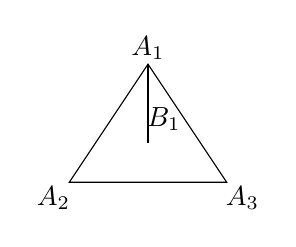
\begin{tikzpicture}
\draw (0,0) -- (2,0) -- (1,1.5) -- cycle;
\node at (1,1.7) {$A_1$};
\node at (-0.2,-0.2) {$A_2$};
\node at (2.2,-0.2) {$A_3$};
\draw (1,0.5) -- (1,1.5);
\node at (1.2,0.8) {$B_1$};
\end{tikzpicture}
\begin{tikzpicture}
\draw[->] (-1.5,0) -- (1.5,0) node[right] {$x$};
\draw[->] (0,-0.5) -- (0,1.5) node[above] {$y$};
\draw (1,0) arc (0:180:1);
\draw (0,0) -- (0.5,0.866);
\end{tikzpicture}
\end{center}

\end{document}
